\chapter{Software}
\label{chap:software}

The third chapter of this thesis describes the web application, CryptoShow, which is developed to provide a user-friendly interface for the methodology described in Chapter~\ref{chap:methodology}. This chapter covers the architecture, technologies used, backend and frontend development, testing, monitoring, and deployment of the application.

\section{Architecture and Used Technologies}
\label{sec:architecture-technologies}

This section outlines the architecture of the CryptoShow application and the technologies employed in its development. The application is designed to be modular and scalable, allowing for easy integration of new features and improvements. For this purpose, we have chosen a service-oritented architecture (SOA) that separates the components, enabling independent development and deployment. The architecture is defined by several Docker containers, each responsible for a specific part of the application. The services are orchestrated using Docker Compose, defined in the \texttt{docker-compose.yml} file, which specifies the services, networks, and volumes required for the application to run. The service architecture is as follows:

\begin{itemize}
    \item \textbf{backend} - Acts as the central API service, facilitating communication between most components. It communicates with Redis, manages API requests from the frontend, and delegates asynchronous tasks to Celery workers. The FastAPI server serves as its entry point. Further details are provided in Section~\ref{sec:backend}.
    \item \textbf{worker-cpu / worker-gpu} - These two services execute asynchronous, resource-intensive tasks without blocking the main FastAPI event loop. \texttt{worker-cpu} runs on the CPU, while \texttt{worker-gpu} leverages GPU acceleration via CUDA when available.
    \item \textbf{frontend} - Delivers the user interface. NginX acts as the gateway to the defined services in Docker Compose and serves static content from a specified directory. Additional information is available in Section~\ref{sec:frontend}.
    \item \textbf{redis} - Functions as the message broker for Celery workers, enabling efficient task distribution.
    \item \textbf{monitoring-flag} - A lightweight service that creates a flag file to enable the monitoring proxy endpoint.
    \item \textbf{remove-monitoring-flag} - A lightweight service that removes the monitoring flag file, disabling the monitoring endpoint.
    \item \textbf{flower} - Provides real-time monitoring and statistics for Celery tasks and queues.
    \item \textbf{celery-exporter} - Exposes Celery metrics to Prometheus, similarly to the Flower service.
    \item \textbf{prometheus} - Collects and stores metrics exported from the Celery workers.
    \item \textbf{grafana} - Offers a user-friendly dashboard for visualizing metrics collected by Prometheus.
\end{itemize}

\begin{figure}[htpb]
    \centering
    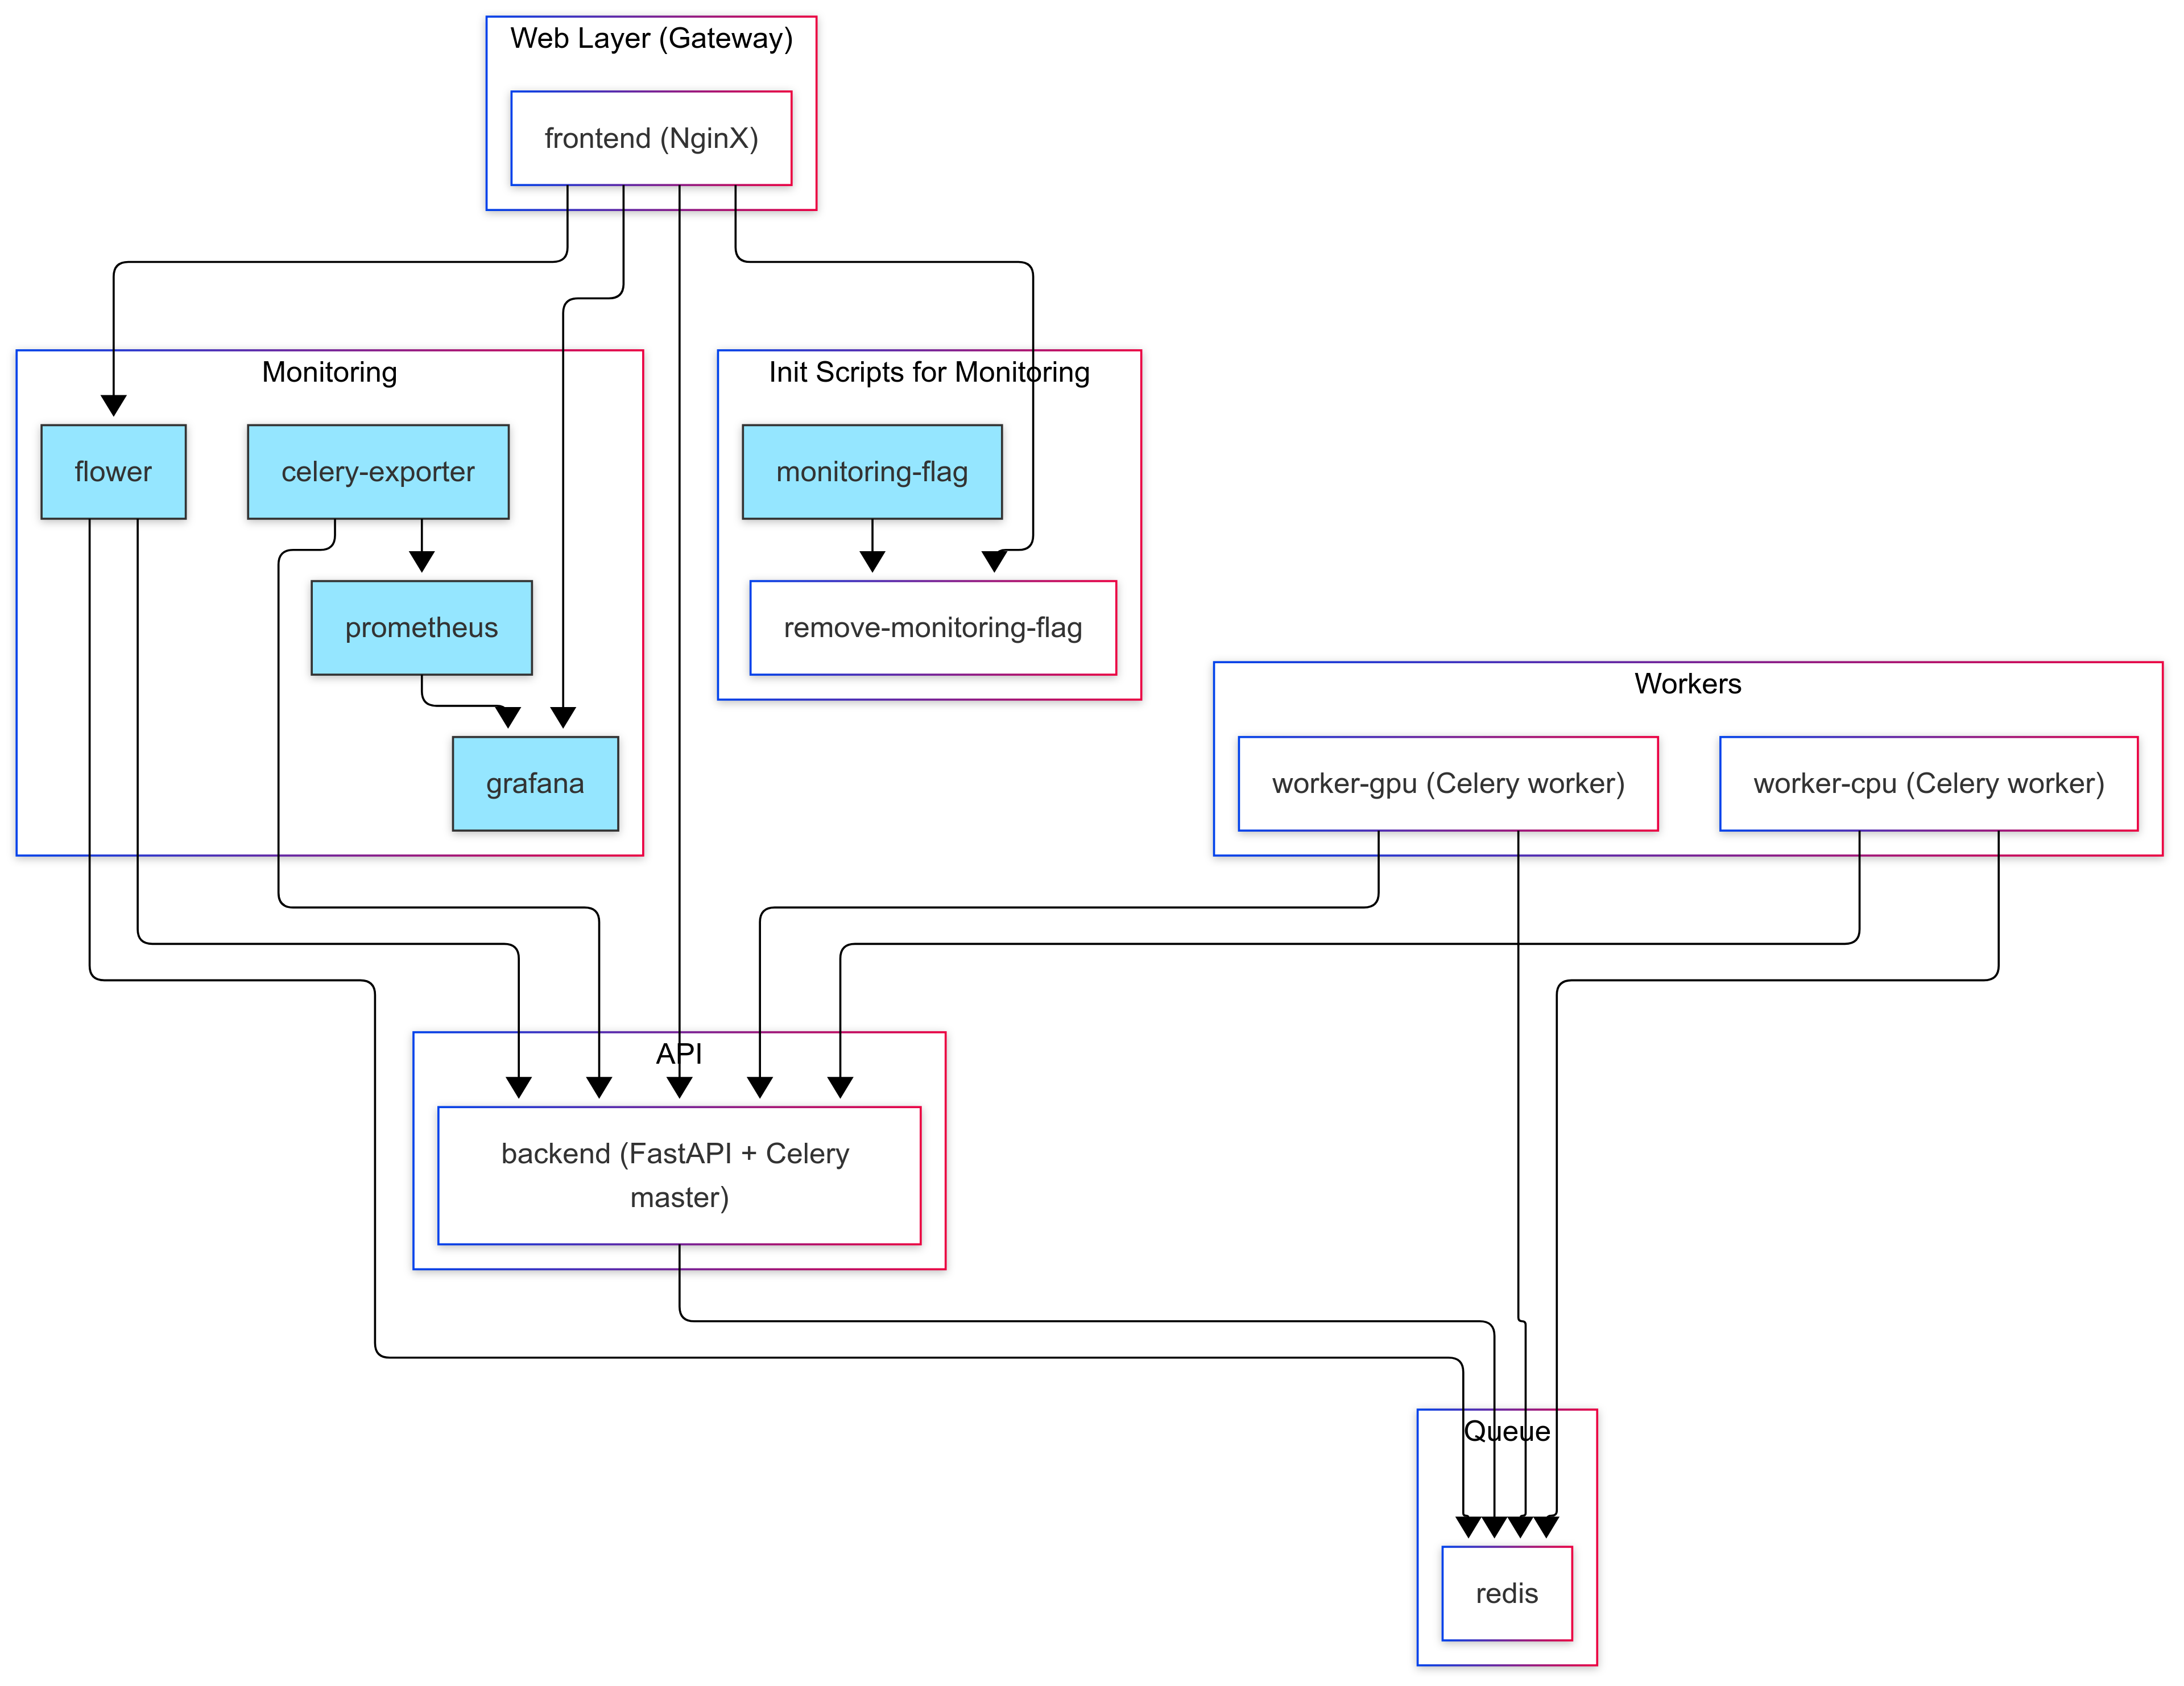
\includegraphics[width=\textwidth]{img/architecture.png}
    \caption{Service architecture of the CryptoShow application. Each small box represents a Docker containerized service. Light blue services are optional, as monitoring is not always required. Arrows indicate communication paths between services. Generated using the Mermaid Chart tool, available at \url{https://www.mermaidchart.com/}.}
    \label{fig:architecture}
\end{figure}

An overview of the service architecture can be seen in Figure~\ref{fig:architecture}. This type of architecture offers a scalable solution that has the potential of easy deployment and development.

Let's also focus on the technology stack for some of the services:

\begin{itemize}
    \item \textbf{backend, worker-cpu / worker-gpu} - Python, notable libraries and tools: Celery (asynchronous tasks in Python), FastAPI, Flower, PyTorch, BioPython, Biotite, Scikit-Learn, MDAnalysis, Gemmi, Redis, uv
    \item \textbf{frontend} - TypeScript, notable libraries, tools and frameworks: React, NginX, Mol*, Bun, Vite
\end{itemize}

The remaining services utilize standard technology stacks commonly associated with their respective functionalities.

\section{Backend}
\label{sec:backend}

\xxx{TODO: add the integration of the developed methodology into the backend}
\xxx{TODO: do we include all API endpoints?}

\subsection{Prediction}
\label{sec:prediction-backend}

\xxx{TODO: reformat this, add more details}
\sloppy
To begin with the prediction, the necessary dependencies for the CryptoBench model must be installed. Once the Python environment is set up, the fine-tuned ESM-2 model (\lstinline!facebook/esm2_t33_650M_UR50D!) is loaded, followed by the corresponding weight file from the Tiny-CryptoBench repository. The protein sequence is then tokenized using the ESM-2 tokenizer, segmented into chunks of 1022 tokens (1024 minus two special tokens), and processed by the CryptoBench model to obtain predictions. These predictions are subsequently concatenated to produce a single prediction vector representing the entire sequence. The model consists of three linear layers, two dropout layers, and a ReLU activation function.

\sloppy
The implementation for this procedure is provided in the \lstinline!backend/prediction/compute_score.py! file. The code is intended for use with individual protein sequences, as it requires parsing and splitting the sequence by chain to ensure accurate predictions.

This code is run asynchronously using Celery workers, allowing efficient processing of multiple sequences in parallel. Moreover, the implementation supports both GPU and CPU execution.

\subsection{Trajectory Animation}
\label{sec:trajectory}

\xxx{TODO: reformat this, add more details}

CryptoShow aims not only to predict and visualize cryptic binding sites, but also to demonstrate potential conformational changes through animated trajectories. To achieve this, we have developed a trajectory animation feature that illustrates structural transitions between related protein conformations.

Let us begin by introducing AHoJ \cite{feidakis2022ahoj} and AHoJ-DB \cite{feidakis2024ahoj} (briefly covered in Section \ref{sec:ahoj}). Apo–Holo Juxtaposition (AHoJ) is a web-based tool designed to identify apo-holo pairs of protein structures within the PDB database (Section~\ref{sec:rcsb-pdb}); currently, querying is limited to this database only.

AHoJ identifies binding residues by spatially marking user-defined ligands using PyMOL (Section~\ref{sec:pymol}). The tool compiles candidate structure chains by detecting UniProt accession numbers and retrieving all chains belonging to the same UniProt AC (Section~\ref{sec:uniprot-db}). It maps binding residues onto the UniProt sequence and examines each candidate chain to determine the presence of mapped binding residues above a minimum threshold. Successful candidates are aligned to the query chain using TM-align \cite{zhang2005tm}, and the area around the superimposed query ligand is examined for ligands. The process classifies each candidate chain as apo or holo based on ligand presence or absence in the defined binding sites, with results visualized in the browser and downloadable for PyMOL analysis. AHoJ-DB is a database of pre-computed apo-holo pairs of protein structures.

For CryptoShow's trajectory animation functionality, we make use of the AHoJ public API to identify apo-holo structural pairs corresponding to the input structure. The query process requires the PDB ID of the input structure\footnote{As mentioned above, AlphaFold structures and custom structures are not supported by AHoJ. Additionally, the input structure may be in holo form. This is not validated in any way. Apo structures are generally more appropriate for this analysis, we leave this decision on the user as it does not affect the functionality of CryptoShow.}, the target chain containing the predicted cryptic binding site, and the central residue of the identified CBS. Listing \ref{lst:ahoj-query} demonstrates the query format. The API response contains all available paired structures, from which users can select any structure to visualize potential conformational transitions. Upon selection, the CryptoShow API initiates the trajectory computation.

\begin{lstlisting}[caption={Sample query format for the AHoJ tool, specifying PDB ID 2src, chain A, aspartic acid residue at position 404}, label={lst:ahoj-query}]
    2src A ASP 404
\end{lstlisting}

First, the target structure for animation is downloaded from AHoJ. Both structure files are then converted to PDB format to ensure each contains only a single model and to allow easier manipulation compared to the mmCIF format (see Section~\ref{sec:pdb-format} and Section~\ref{sec:mmcif-format}). Subsequently, the PDB file is processed using the MDAnalysis library \cite{gowers2019mdanalysis}, from which the sequence and corresponding residues are extracted. At this point, we have obtained the necessary structural information.

Next, we need to determine which residues should be included in the animation. To achieve this, we employ a straightforward approach by computing the longest common subsequence of both protein sequences \xxx{TODO: should I add pseudocode here? it's not really that hard...}. This ensures that only residues present in both structures are animated. The subsequence length must be greater than zero due to the inherent logic of AHoJ. Once the common subsequence is identified, we extract the corresponding residues from both structures. We utilize the MDAnalysis library to perform this operation at the atomic level, as PDB files store coordinates for individual atoms rather than residues. Additionally, we extract all ligands from both structures to include them in the final animation.

In the end, we generate the trajectory using cubic spline interpolation \cite{mckinley1998cubic} implemented in the SciPy library \cite{virtanen2020scipy}. We create a trimmed PDB file containing only the relevant residues and ligands, along with a trajectory file featuring interpolated coordinates across a predetermined number of frames (set arbitrarily to 50). The final visualization presents the original structure at 50\% opacity and the target holo structure at full opacity, as illustrated in Figure \ref{fig:trajectory-animation}.

\begin{figure}[htbp]
    \centering
    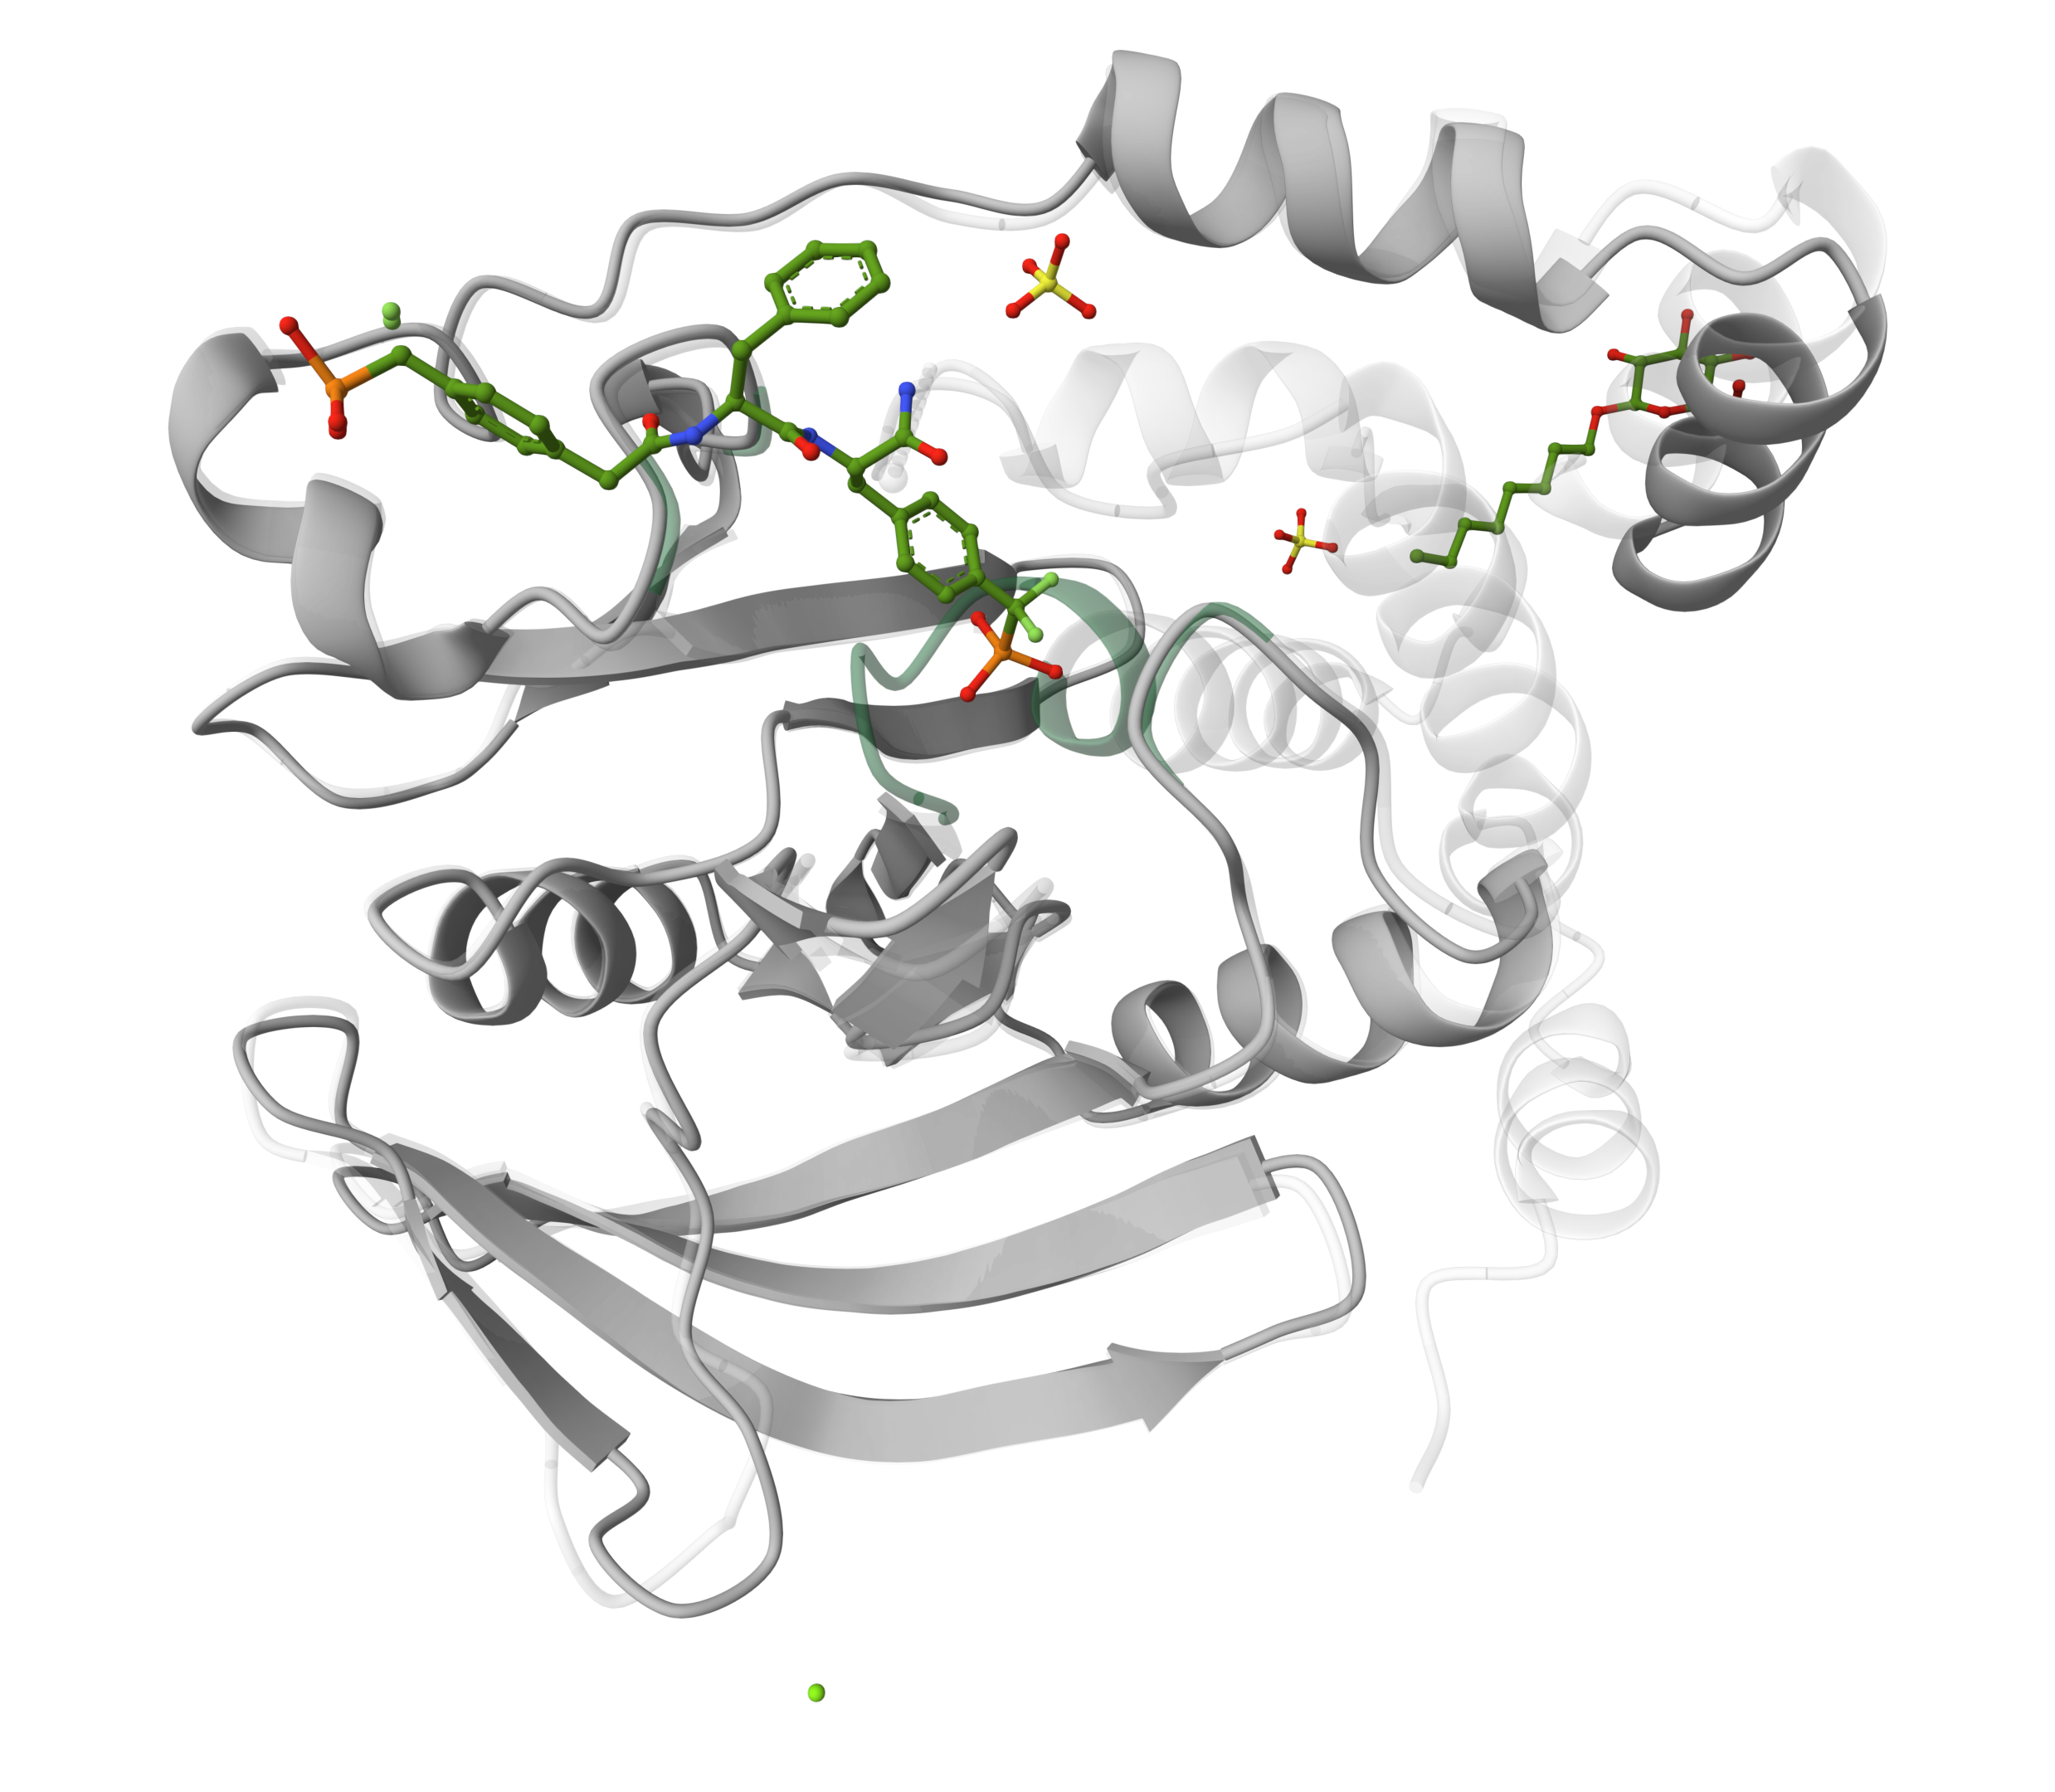
\includegraphics[width=\textwidth]{img/trajectory_animation.png}
    \caption{Example of trajectory animation demonstrating conformational changes between the input structure 1PTY (Crystal Structure of Protein Tyrosine Phosphatase 1B Complexed with Two Phosphotyrosine Molecules) and 2CNE (Structural Insights into the Design of Nonpeptidic Isothiazolidinone - Containing Inhibitors of Protein Tyrosine Phosphatase 1B). The input structure is displayed with 50\% transparency, while the target holo structure is rendered at full opacity. The ligand is represented in ball-and-stick format. Visualized using Mol* in CryptoShow.}
    \label{fig:trajectory-animation}
\end{figure}
Although this process generates a trajectory, it is important to note that this represents only a simple interpolation of residue coordinates. The trajectory does not depict actual conformational changes, but rather provides a smooth transition between the two structures. To capture genuine conformational dynamics, one would need to perform molecular dynamics simulations, which are computationally intensive and require significant time investment \cite{schlitter1993targeted}.

The source code for the trajectory animation functionality can be found in the \lstinline!backend/trajectory_generator! directory. As with the prediction and clustering components, the implementation details in the actual pipeline will be covered in Chapter \ref{chap:software}.


\section{Frontend}
\label{sec:frontend}

\xxx{TODO: describe both frontend overall and the Mol* specifics, including information about the trajectory animation}


\section{Tests and Monitoring}
\label{sec:tests-monitoring}

\xxx{TODO: add information about Docker healthchecks, monitoring options, Grafana, Prometheus, Flower}


\section{Deployment}
\label{sec:deployment}

\xxx{TODO: describe options for Docker, mention open ports, instructions, maybe requirements for the server}
